%%
%% Meta: TI nSpire Einführung
%%       Ziel: Damit die Grundoperationen damit durchgeführt werden können.
%%             Damit man sich an den Rechner gewöhnt.
%%

\input{bbwLayoutPage}

%%%%%%%%%%%%%%%%%%%%%%%%%%%%%%%%%%%%%%%%%%%%%%%%%%%%%%%%%%%%%%%%%%

\usepackage{amssymb} %% für \blacktriangleright
\renewcommand{\metaHeaderLine}{Arbeitsblatt}
\renewcommand{\arbeitsblattTitel}{Aufgaben zu trigonometrischen Funktionen}

\begin{document}%%
\arbeitsblattHeader{}


\begin{center}
\raisebox{-1cm}{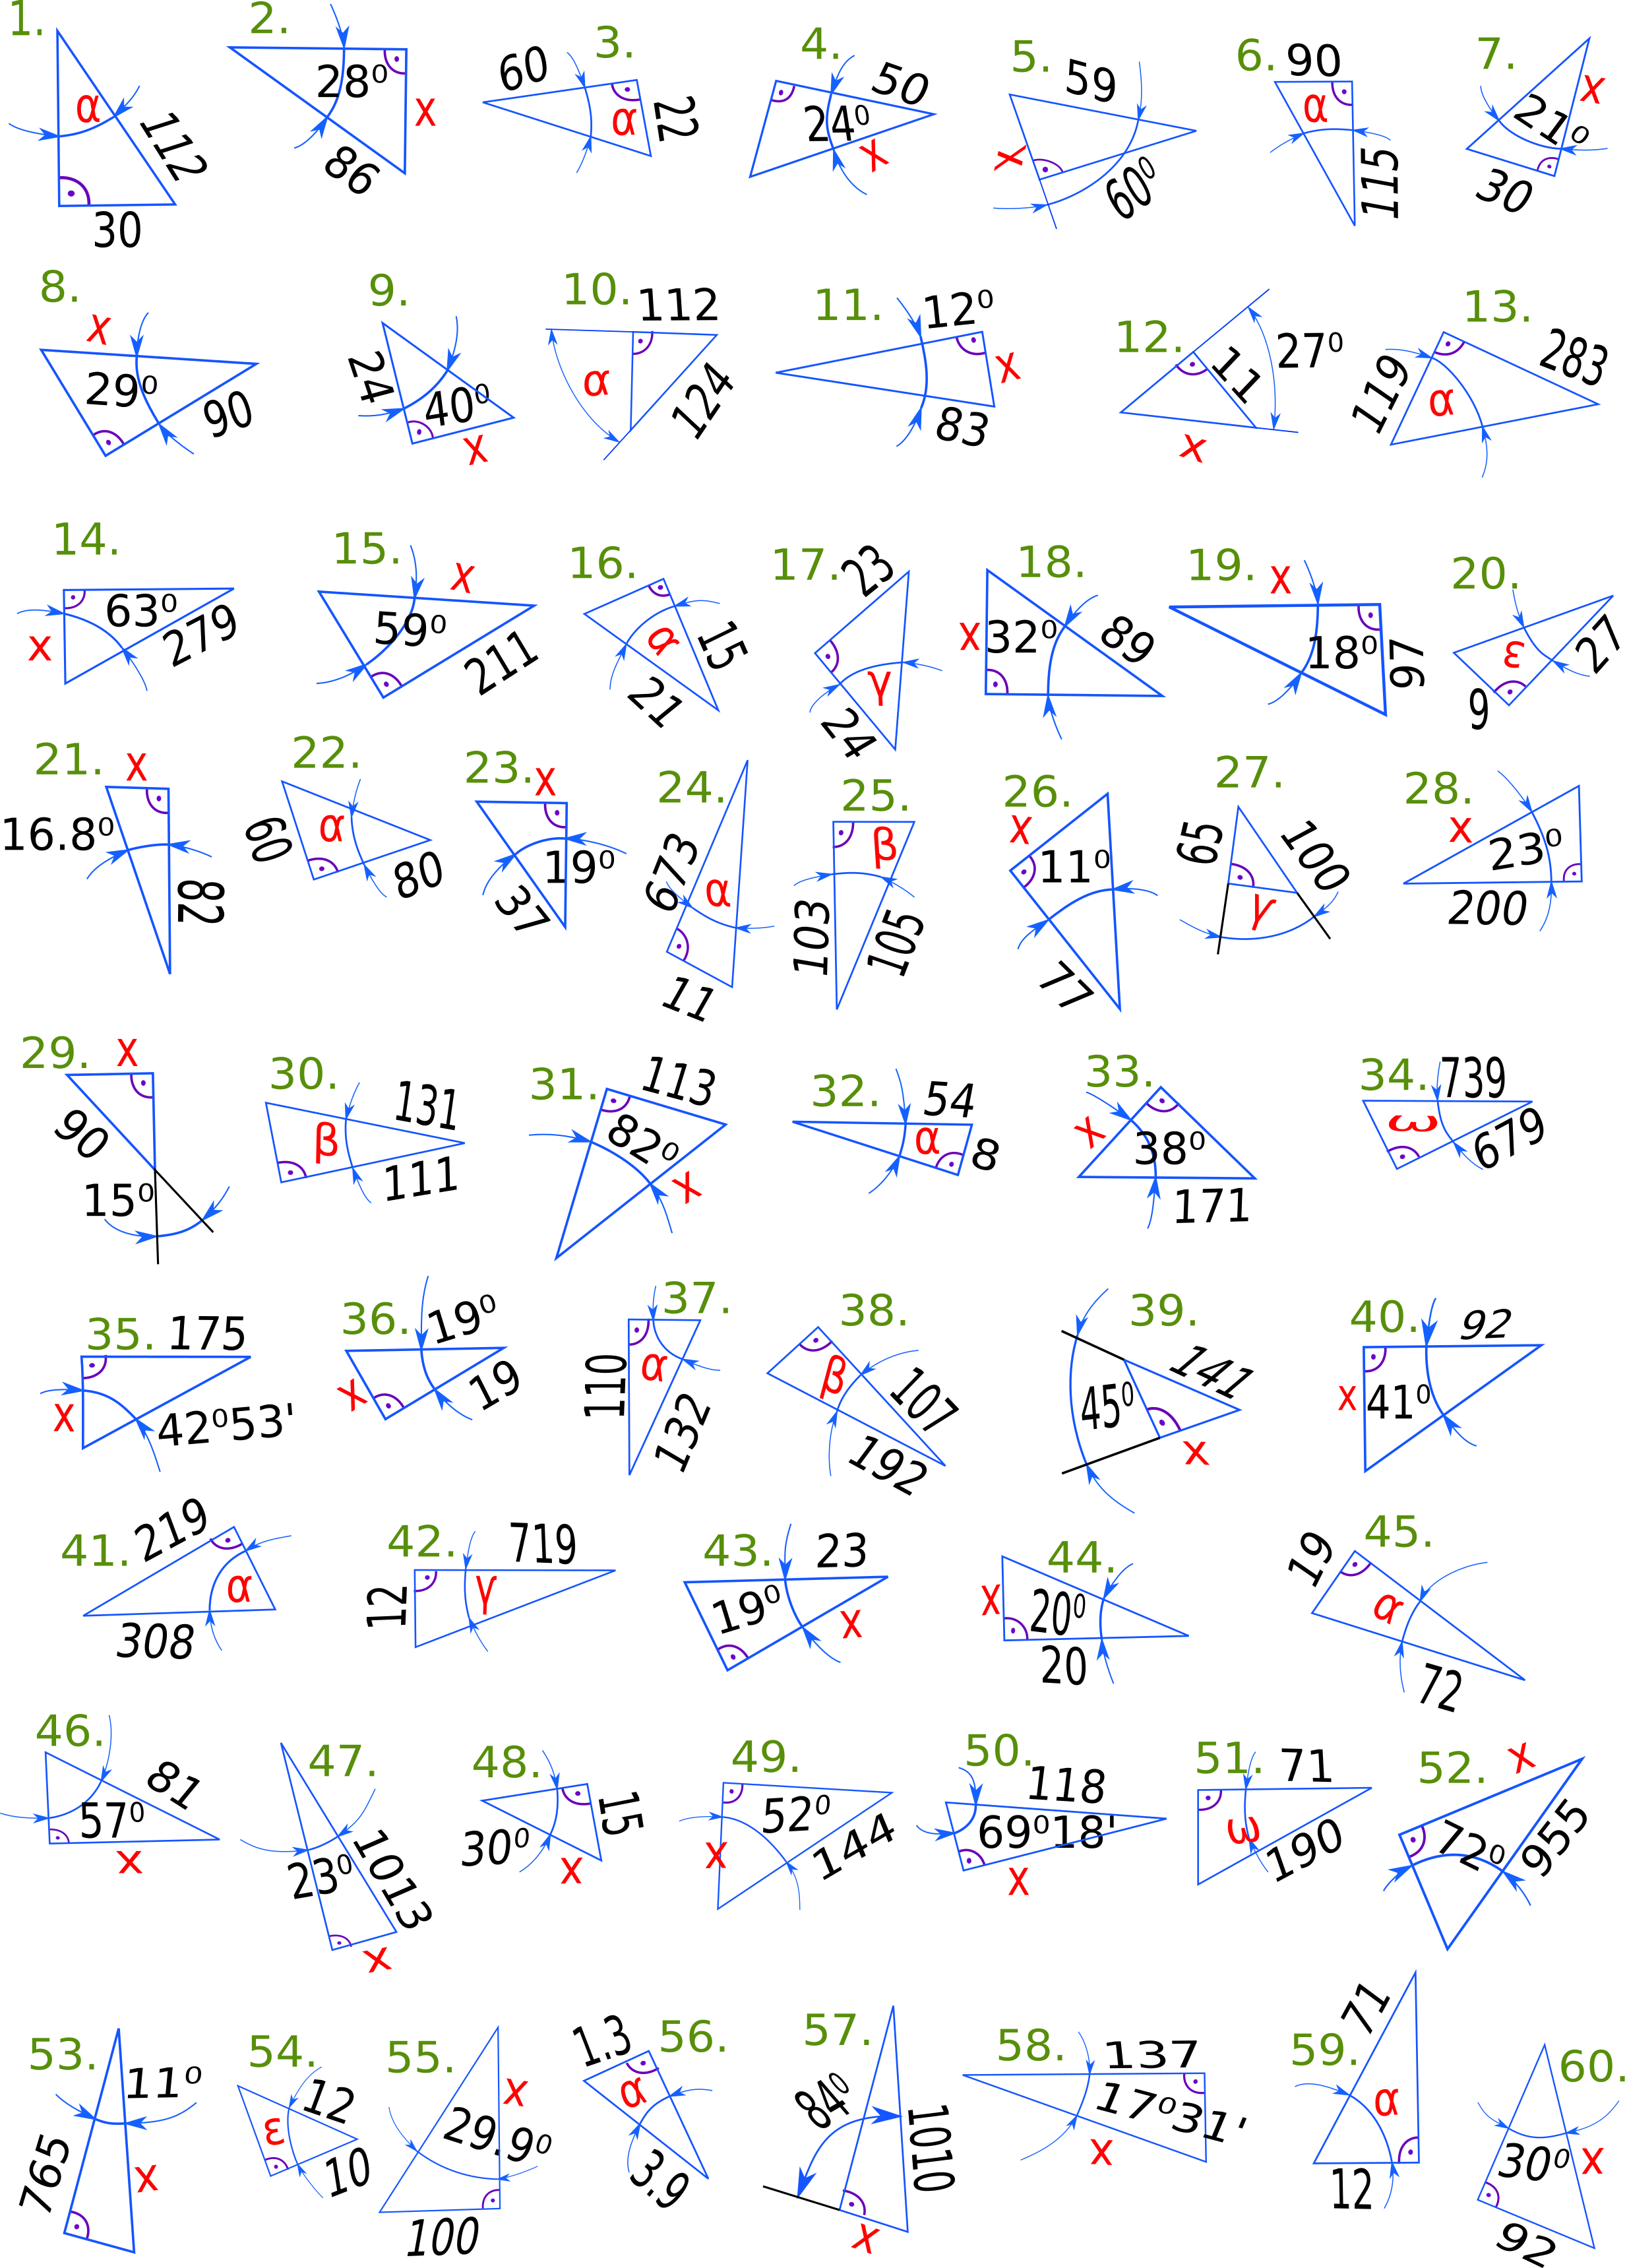
\includegraphics[width=16.5cm]{img/v2020.png}}
\end{center}



\end{document}
